\documentclass[oneside, 11pt]{article}

\usepackage[T1]{fontenc}
\usepackage[utf8]{inputenc}
\usepackage[english]{babel}
\usepackage{enumerate}
\usepackage{isotope}


\usepackage{fouriernc}
\usepackage[detect-all, binary-units, separate-uncertainty=true,
            per-mode=symbol, retain-explicit-plus, retain-unity-mantissa=false]{siunitx}

\usepackage{setspace}
\setstretch{1.2}

\setlength{\parskip}{\smallskipamount}
\setlength{\parindent}{0pt}

\usepackage[headheight=14pt]{geometry}
\geometry{marginparwidth=0.5cm, verbose, a4paper, tmargin=3cm, bmargin=3cm,
          lmargin=2cm, rmargin=2cm}

\usepackage{float}

\usepackage[fleqn]{amsmath}
\numberwithin{equation}{section}
\numberwithin{figure}{section}

\usepackage{graphicx}
\graphicspath{{images/}{../../../images/}}

\usepackage{tikz}
\usetikzlibrary{shapes}
\usetikzlibrary{plotmarks}

\newcounter{Exercise}
\setcounter{Exercise}{1}
\usepackage{xcolor}
\definecolor{shadecolor}{gray}{0.9}
\usepackage{framed}
\usepackage{caption}

\usepackage{url}


\usepackage{fancyhdr}
\pagestyle{fancy}
\fancyhf{}
\rhead{\thepage}
\renewcommand{\footrulewidth}{0pt}
\renewcommand{\headrulewidth}{0pt}

\fancypagestyle{firststyle}
{
    \fancyhf{}
    \rhead{\thepage}
    \cfoot{\includegraphics[height=30pt]{HiSPARClogo}}
    \rfoot{\includegraphics[height=25pt]{CCbysa}}
    \lfoot{
\includegraphics[height=30pt]{NIKHEFlogo}}
    \renewcommand{\footskip}{50pt}
    \renewcommand{\footrulewidth}{0.1pt}
    \renewcommand{\headrulewidth}{0pt}
}

\newcommand{\figref}[1]{Figuur~\ref{#1}}

\newcommand{\hisparc}{\textsmaller{HiSPARC}\xspace}
\newcommand{\kascade}{\textsmaller{KASCADE}\xspace}
\newcommand{\sapphire}{\textsmaller{SAPPHiRE}\xspace}
\newcommand{\jsparc}{\textsmaller{jSparc}\xspace}
\newcommand{\hdf}{\textsmaller{HDF5}\xspace}
\newcommand{\aires}{\textsmaller{AIRES}\xspace}
\newcommand{\csv}{\textsmaller{CSV}\xspace}
\newcommand{\python}{\textsmaller{PYTHON}\xspace}
\newcommand{\corsika}{\textsmaller{CORSIKA}\xspace}
\newcommand{\labview}{\textsmaller{LabVIEW}\xspace}
\newcommand{\daq}{\textsmaller{DAQ}\xspace}
\newcommand{\adc}{\textsmaller{ADC}\xspace}
\newcommand{\hi}{\textsc{h i}\xspace}
\newcommand{\hii}{\textsc{h ii}\xspace}
\newcommand{\mip}{\textsmaller{MIP}\xspace}
\newcommand{\hisparcii}{\textsmaller{HiSPARC II}\xspace}
\newcommand{\hisparciii}{\textsmaller{HiSPARC III}\xspace}

\DeclareSIUnit{\electronvolt}{\ensuremath{\mathrm{e\!\!\:V}}}

\DeclareSIUnit{\unitsigma}{\ensuremath{\sigma}}
\DeclareSIUnit{\mip}{\textsmaller{MIP}}
\DeclareSIUnit{\adc}{\textsmaller{ADC}}

\DeclareSIUnit{\gauss}{G}
\DeclareSIUnit{\parsec}{pc}
\DeclareSIUnit{\year}{yr}




%document details
\author{Koos Kortland \\ translated and adapted by K. Schadenberg}
\date{}
\title{HiSPARC Detector - Single Detector}


\begin{document}
\maketitle

\section{Introduction}
This module is the first in a series describing the HiSPARC detector. A complete detector station consists of two or four detectors, a GPS antenna, an electronics box, and a computer. In this module we will take a closer look at the heart of the station; the detector. 

\section{HiSPARC Detector}
The HiSPARC detector consists of three parts: a scintillator plate, a light guide, and a photomultiplier tube (PMT). Figure~\ref{fig:detector} shows how these three components are connected together.

The scintillator plate is made from a plastic mixed with an organic compound which creates light (photons) when a charged particle passes through the plate.\footnote{In de module `Fluorescence' and `de Broglie' you can read more about this scintillating effect.} The intensity of this flash of light is proportional to the amount of energy deposited inside the plate.

\begin{figure}\begin{center}
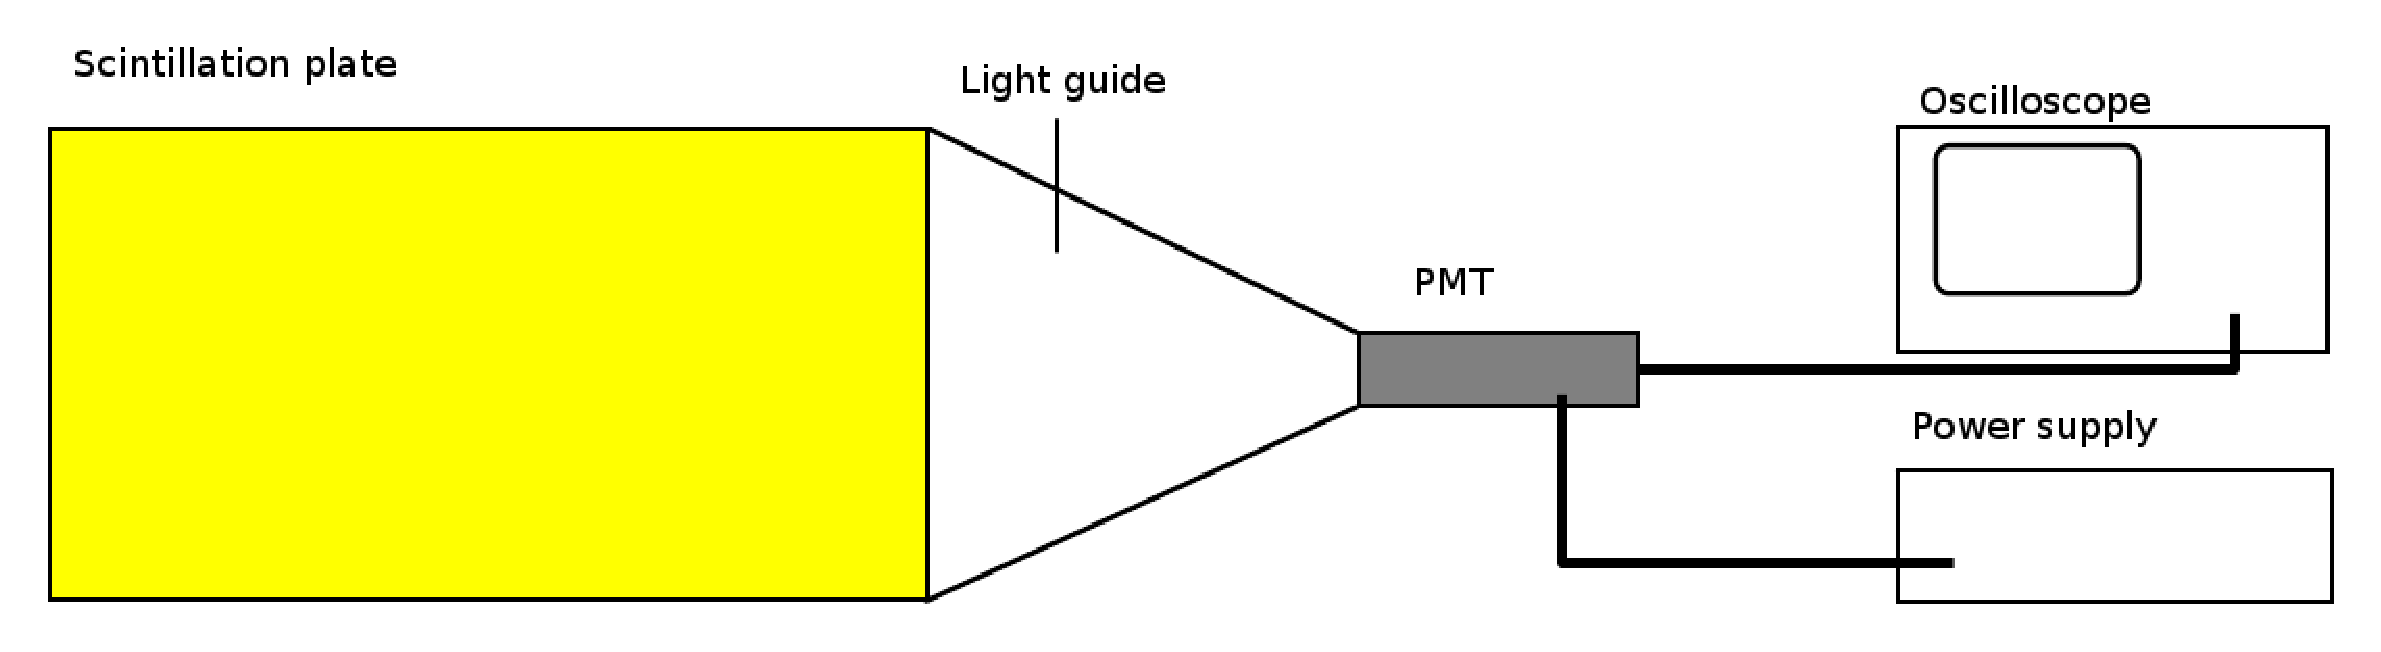
\includegraphics[scale=0.38]{detector}%
\caption{A single HISPARC detector consists of a scintillator plate roughly 1 metre long and half a metre wide connected to a light guide. This light guide `guides' the light created inside the plate to the much smaller photomultiplier tube (PMT). The PMT operates at a high voltages supplied by power supply. The current created by the PMT is measured by a oscilloscope.}\label{fig:detector}
\end{center}\end{figure}

Some of the created photons will travel via the light guide to the PMT. Here the light is converted into a stream of electrons; a measurable electrical current. This electrical pulse as measured by the oscilloscope is shown in figure~\ref{fig:scope}.

\begin{figure}\begin{center}
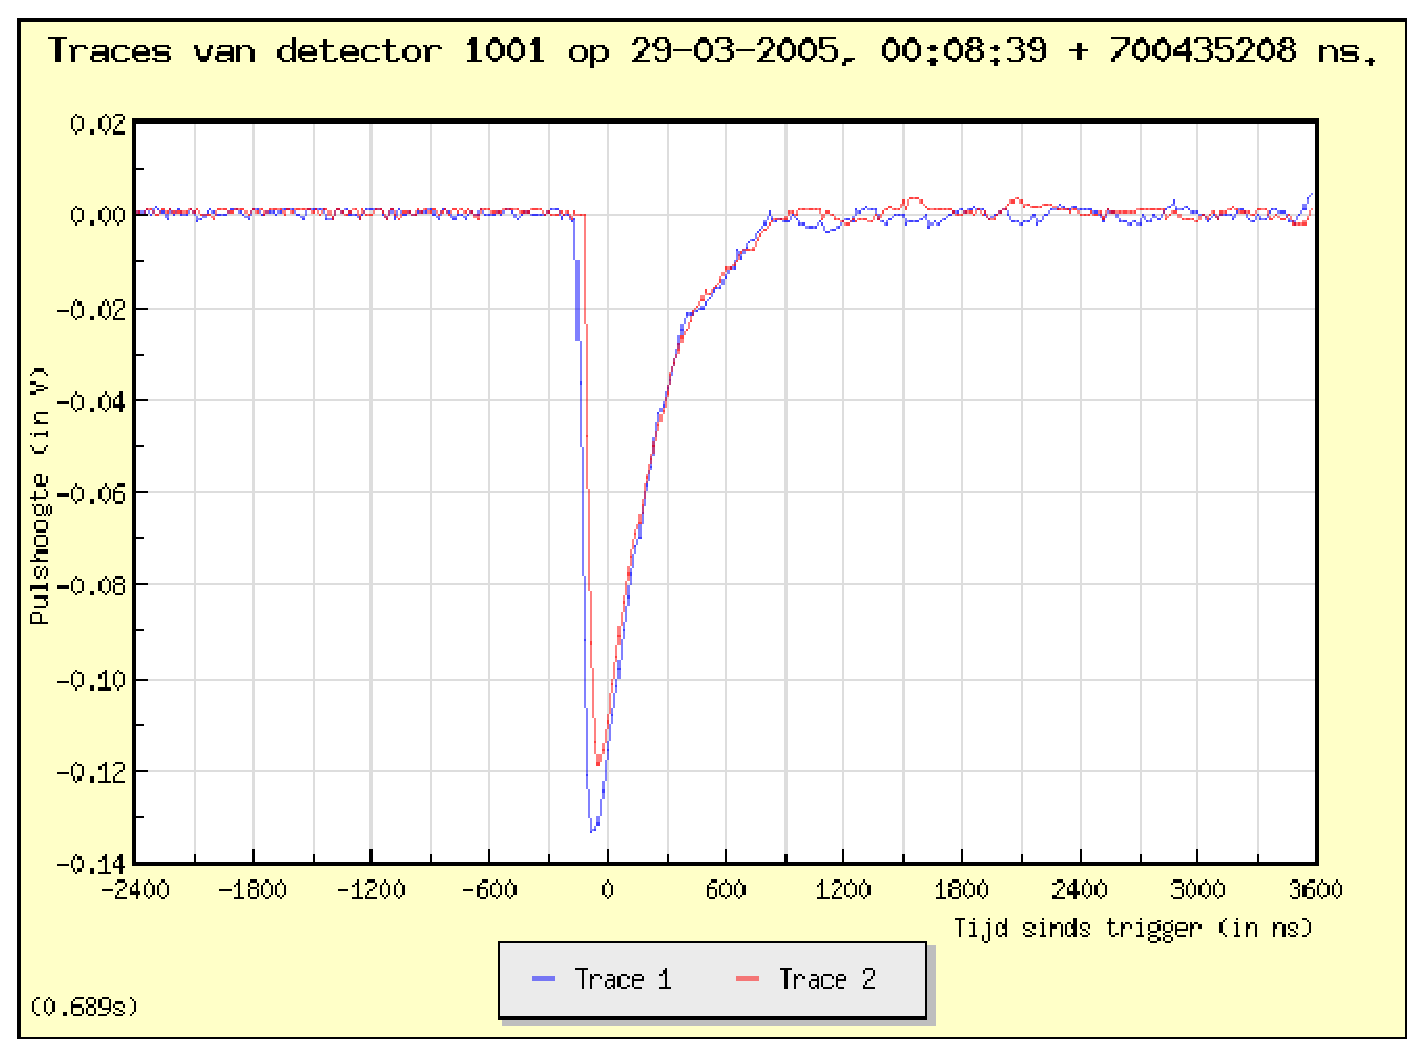
\includegraphics[scale=0.45]{scope}%
\caption{Example of the voltage pulse created by the PMT after the passage of a muon, as seen by the oscilloscope. This figure shows two peaks of roughly the same size, created by two detectors connected to the same detector station.\protect\footnotemark ~The scaling in this graph has been changed to make the peaks more clearly visible. In reality every division (space between two vertical lines) is only 3~ns, a hundred times smaller than displayed.}\label{fig:scope}
\end{center}\end{figure}
\footnotetext{See `HiSPARC Detector - Detector Station' for more details.}

What can we learn from the shape of this electrical pulse? To answer this question we will first take a look at what we would expect to measure when a particle passes through the detector. We will answer the following questions related to the different steps inside the detector transforming a muon into a measurable current:
\begin{itemize}
\item How much energy is lost by a muon travelling through the detector?
\item How many photons can be (are) created by the deposited energy?
\item How large is the fraction of photons reaching the PMT?
\item How many electrons are created by the PMT after the arrival of the photons?
\item How large is the voltage measured by the oscilloscope created by this current?
\end{itemize}

\section{Detector Signal}
We will answer the questions stated above one by one.
\subsection{Energy deposition}
Figure~\ref{fig:energy_loss} shows the amount of energy lost by a muon when it interacts with matter such as the scintillation plate. This energy loss $\Delta E$ is given in MeV/(g/cm$^2$). Not the most common unit, certainly not for energy. The energy loss of the muon during interaction with other matter is dependent on the density $\rho$ of the material and the path length $l$ of the muon through the material. The larger the density or path length, the larger the energy loss. The energy loss is directly proportional to the product of the density and path length:
\begin{equation}
\Delta E = k \cdot \rho \cdot l
\end{equation}
with $k$ a constant whose value is dependent on the type of material (but varies only very slightly).

The unit of the product $\rho \cdot l$ is grams per centimetre squared (g/cm$^2$). Because energy, $\Delta E$, should have the unit eV (or Joules or equivalent), the unit for the constant $k$ is MeV/(g/cm$^2$). The graph in figure~\ref{fig:energy_loss} therefore does not shown the energy loss but rather the value of $k$:
\begin{equation}
k = \frac{\Delta E}{\rho l }
\end{equation}
Because $k$ only varies slightly with different materials the graph in figure~\ref{fig:energy_loss} is valid for most materials.

Figure~\ref{fig:energy_loss} also shows that the energy loss is proportional to the energy $E$. Low and very high energetic muons lose more energy than intermediate muons. The muons created in air showers, the ones we are interested in, have energies in the order of GeVs ($10^9$~eV).

\begin{figure}\begin{center}
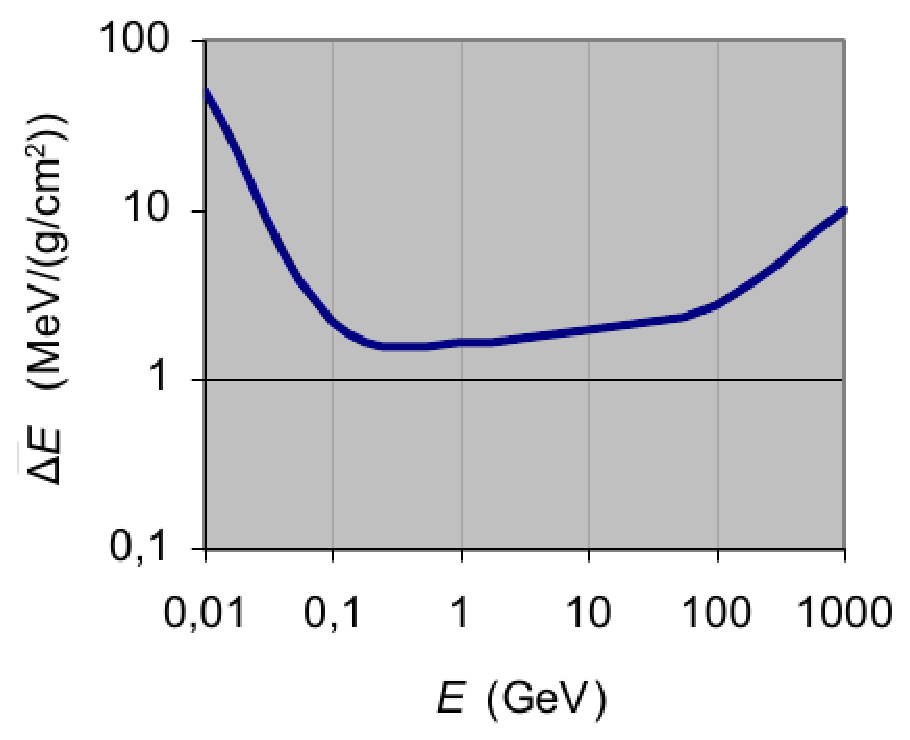
\includegraphics[scale=0.5]{energy_loss}%
\caption{The energy loss $\Delta E$ of muons during interactions with other matter as a function of the muon-energy $E$.}\label{fig:energy_loss}
\end{center}\end{figure}

\begin{shaded}
\textbf{Exercise \theExercise \stepcounter{Exercise}} : The energy loss of a muon inside the HiSPARC detector depends on the material properties of the scintillator plate. HiSPARC uses a 2~cm thick plate with a density of 1~g/cm$^3$. Calculate the energy loss, in MeV, of a perpendicular incident muon.\end{shaded}

The number of photons created by a passing muon is determined by the energy loss of the muon and the energy needed to create a single photon. The last is a material property.\footnote{See `Fluorescence' for more details.} The scintillator plate HiSPARC uses creates blue light which has an energy of roughly 3~eV. However, 100~eV is needed to create one photon. 

\begin{shaded}
\textbf{Exercise \theExercise \stepcounter{Exercise}} :  Use your previous answer to calculate the number of photons created by a passing muon, $N_p$.\end{shaded}

To calculate the number of photons created by the scintillator plate we used the  graph in figure~\ref{fig:energy_loss}. However, this graph shows an average energy deposition. The actual energy loss $\Delta E$ of a muon is sometimes a bit higher and sometimes a bit lower. This is because this deposition of energy is a statistical process. The exact distribution of different amounts of energy deposition was determined by Lev Landau in 1944. The distribution function describing this process is named after him: the Landau-distribution.

The Landau-distribution for muons is shown in figure~\ref{fig:energy_landau}. This graph shows the number of muons $N$ which deposit a certain amount of energy $\Delta E$. The distribution shows one clear peak value, the most probable (or most frequent) energy loss. This is the value used to create figure~\ref{fig:energy_loss}.

\begin{figure}[b]\begin{center}
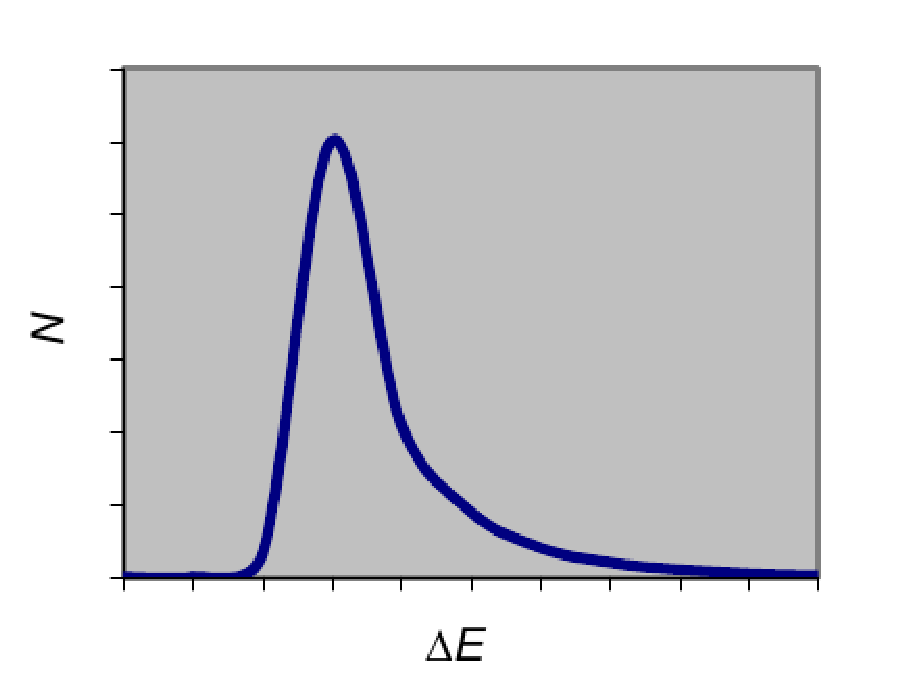
\includegraphics[scale=0.4]{energy_landau}%
\caption{Landau distribution of the energy loss $\Delta E$ of a large number of muons.}\label{fig:energy_landau}
\end{center}\end{figure}

Because the amount of energy deposited in the scintillator plate varies with every muon, the number of created photons also differs. This in turn affects the voltage pulse created by the PMT. If we were to make a graph of the different voltage pulses created by a large number of muons we expect to see a Landau-distribution.

\subsection{Loss of Photons}
We have calculated that the number of photons created by a passing muon, $N_p$, is roughly $4 \cdot 10^4$. The next question we need to answer is how many of these photons reach the cathode of the PMT; $N_{p,C}$? Or, in other words, how many of the created photons are lost inside the scintillator and light guide? Unfortunately we can only make a rough estimation of this number.

The main cause of the loss of light is the refraction and reflection of light on the edges of the detector. Figure~\ref{fig:refraction} shows a side view of the scintillator plate. The source of the light is shown as a single point placed roughly in the centre of the plate. Part of the created light will stay within the plate due to total internal reflection at the edges of the detector, the other part is lost.

\begin{shaded}
\textbf{Exercise \theExercise \stepcounter{Exercise}} :
\begin{enumerate}[-]
\item Describe in your own words the phenomenon of total internal reflection; what is it and when does it occur? Make sure to use the following term in your answer: refraction, angle of incidence, critical angle, and refractive index.
\item The scintillation material has a refractive index $n=1.58$. Calculate the critical angle for this material.
\item Explain that in the 2-dimensional situation of figure~\ref{fig:refraction} roughly half of the created photons most definitely will not reach the PMT.
\item Explain how in a 3-dimensional situation an even larger part of the photons will not reach the PMT. (Do not forget to include the effect of absorption in your answer.)
\item Explain how the geometry of light guide between the scintillator plate and PMT (see figure~\ref{fig:detector}) causes a further loss of photons.
\item Assume that the amount of photons reaching the PMT is 1\%. Calculate the number of photons $N_{p,C}$ hitting the PMT-cathode after the passage of the muon
\end{enumerate}
\end{shaded}

\begin{figure}\begin{center}
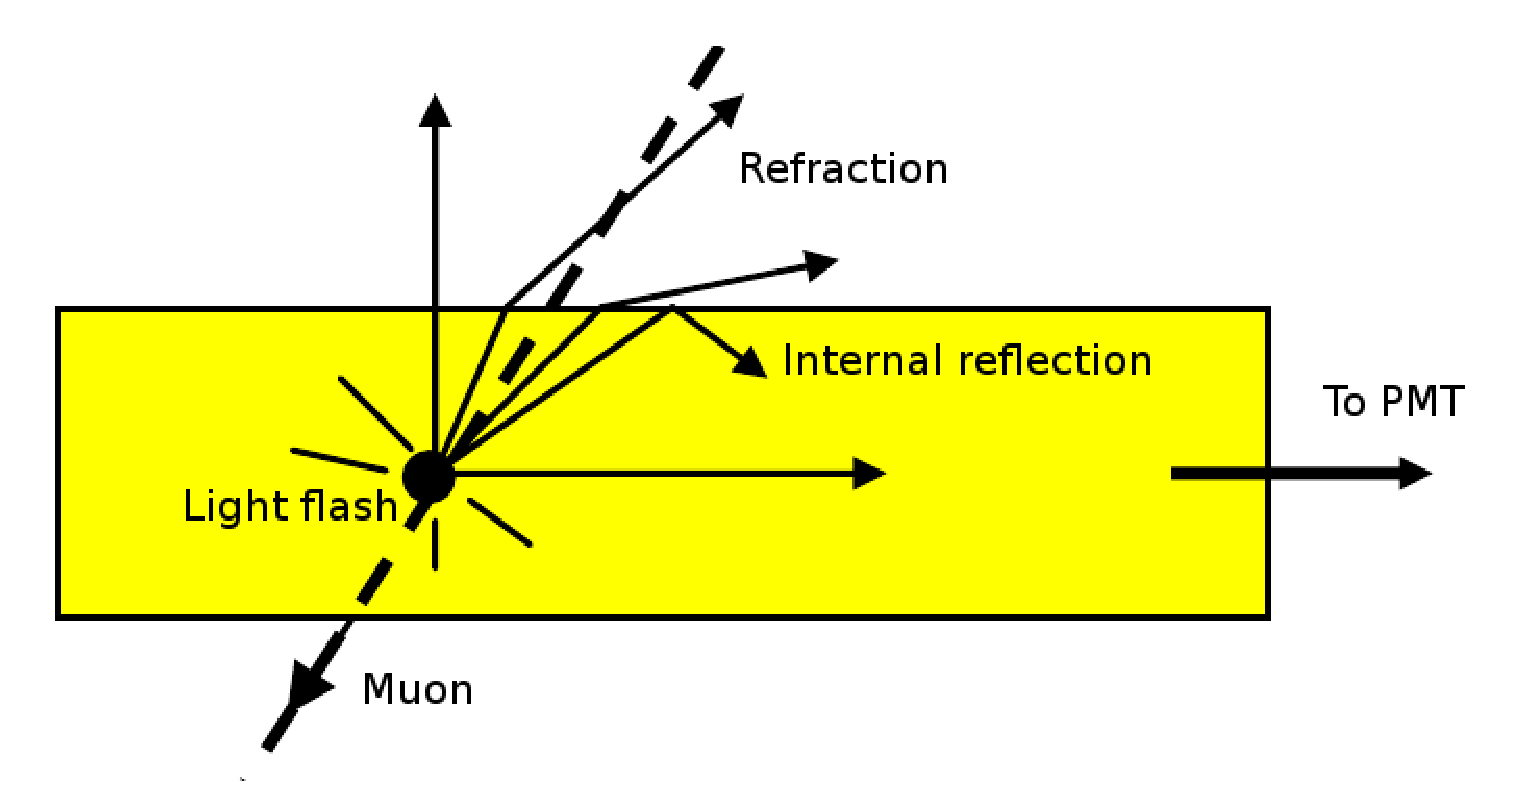
\includegraphics[scale=0.5]{refraction}%
\caption{Cross section of the scintillator in side view. In this greatly simplified situation a passing muon creates a flash of light in a single point.}\label{fig:refraction}
\end{center}\end{figure}

Total internal reflection keeps a part of the photons inside the scintillator plate and light guide. However only a very small part of the photons will reach the PMT. Some are absorbed by the material, but most are lost by refraction at the detector edges. We can reduce this loss of photons by adding a reflective layer to the detector, reflecting the photons back into the detector. This reflective layer is aluminium foil, the reflection however is less than perfect. We will therefore keep our assumption that only 1\% of the created photons reaches the PMT.

\subsection{Electron Gain}
The PMT transforms the flash of light created by the scintillator plate into an electrical signal. Or to use a more exact phrasing: when a number of photons enters the PMT, it will produce a number of electrons. This stream of electrons, an electrical current, can be made visible using an oscilloscope.

Only 1\% of the created photons, $N_p=4 \cdot 10^4$, reaches the PMT, $N_{p,C}=4 \cdot 10^2$. The question now before us is how many electrons, $N_{e,A}$, are produced at the anode of the PMT because of this. The PMT not only converts photons into electrons, it is also a very powerful amplifier. The number of electrons produced can be far greater than the number of incident photons. In the next exercise we will take a look at how large this number can be.

\begin{shaded}
\textbf{Exercise \theExercise \stepcounter{Exercise}} : Figure~\ref{fig:PMT_cross_section} shows the internal components of a PMT. Use this figure to describe how a PMT works; how does the PMT convert photons into electrons, how is the number of electrons amplified, what drives the electrons from the cathode to the anode? Also explain the importance of the voltage across the PMT and how it influences the gain (amplification).\\
\emph{Hint: You might need to do a bit of online research to answer all the questions above. A nice simulation of a PMT can be found at:\\}
\url{http://micro.magnet.fsu.edu/primer/flash/photomultiplier/}
\end{shaded}

\begin{figure}\begin{center}
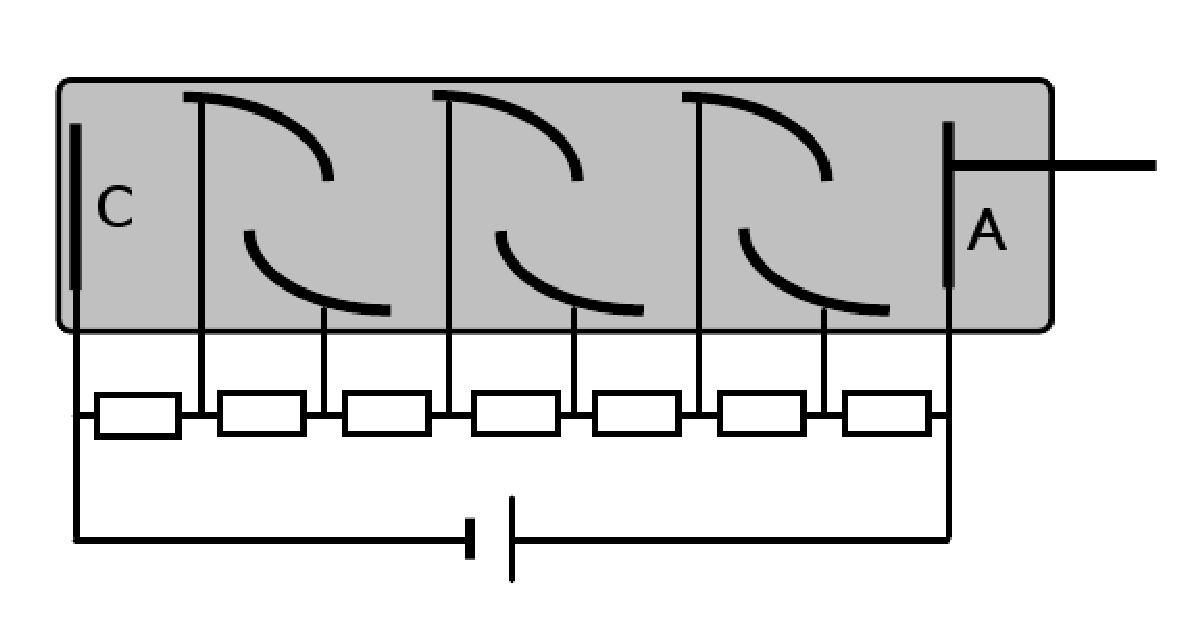
\includegraphics[scale=0.38]{PMT_cross_section}%
\caption{Cross section of a Photo Multiplier Tube (PMT).}\label{fig:PMT_cross_section}
\end{center}\end{figure}

\begin{shaded}
\textbf{Exercise \theExercise \stepcounter{Exercise}} : The PMTs used by HiSPARC have the following specifications according to the manufacturer:
\begin{description}
\item [Quantum efficiency $\eta$ 0.28 (28\%)] If a hundred photons hit the first stage of the PMT, the cathode, only 28 will create a free electron.
\item [Nominal gain G $ \mathbf{3 \cdot 10^6}$] The gain of a PMT is dependent on the voltage across the different dynode stages, but the nominal value is $3 \cdot 10^6$; every free electron at the PMT-cathode will result in $3 \cdot 10^6$ electrons at the PMT-anode.
\end{description}
Use the values above to calculate the number of electrons at the PMT-anode, $N_{e,A}$ after the passage of a muon.
\end{shaded}

\subsection{Pulse Height}
If you have done your sums right you now know that the passage of a single muon causes the `delivery' of $3.4 \cdot 10^9$ electrons at the PMT-anode. Figure~\ref{fig:PMT_connection} shows how the PMT is connected to the oscilloscope, the electrons can flow to the ground via a $50~\Omega$ resistor. This setup allows us to measure the stream of electrons as a voltage pulse.

\begin{figure}\begin{center}
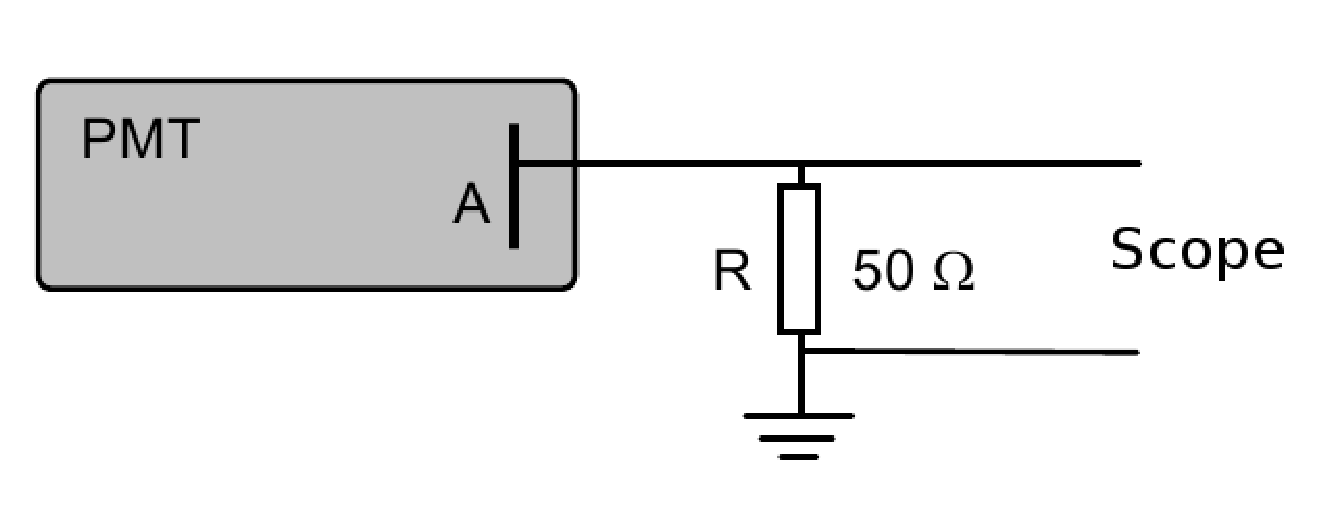
\includegraphics[scale=0.38]{PMT_connection}%
\caption{The PMT-signal is carried to the oscilloscope via a resistor. }\label{fig:PMT_connection}
\end{center}\end{figure}

\begin{shaded}
\textbf{Exercise \theExercise \stepcounter{Exercise}} : Figure~\ref{fig:scope} shows the voltage pulse as seen on the oscilloscope screen.
\begin{enumerate}[-]
\item Determine the duration of the pulse in figure~\ref{fig:scope} and use this to calculate the (average) current $I$ in the resistor $R$.
\item Calculate the (average) voltage $U$ across resistor $R$. Compare your calculated value with the height in figure~\ref{fig:scope}. Explain if both are in agreement.
\item What are the most important uncertainties in your calculation of the (theoretical) expected pulse height?
\end{enumerate}
\end{shaded}

\begin{shaded}
\textbf{Exercise \theExercise \stepcounter{Exercise}} : The result of a large number of muon-detections can be shown in a pulse height histogram. The number of events $N$ is plotted on the vertical axis as a function of the pulse height $U$, measured in mV, plotted on the horizontal axis.

Sketch the expected pulse heigh histogram for a large number of muon-detections. Explain the shape of your histogram.
\end{shaded}

\begin{shaded}
\textbf{Exercise \theExercise \stepcounter{Exercise}} : Assume that there is a way to only record the pulses created by muons passing through a small portion (say 10~cm$^2$) of the entire scintillator plate surface. Draw the expected pulse height histograms for a large number of muons for at least two different locations on the scintillator plate. Explain the differences and/or similarities between the two histograms.\end{shaded}

\begin{shaded}
\textbf{Exercise \theExercise \stepcounter{Exercise}} : How would you select or record the pulses as described in the previous exercise?\end{shaded}

\end{document}

